\acs{LBM} est un algorithme propice pour des simulations distribuées sur les nœuds d'un \textit{cluster} de calcul, ou sur les cœurs d'un \acs{GPU}. Il a par conséquent attiré l'attention de nombreux chercheurs. 

Ce chapitre fait un tour d'horizon des technologies et des méthodes utilisées pour améliorer les performances des simulations basées sur la méthode de Lattice Boltzmann. Les sections suivantes présentent les travaux chronologiquement, en commençant par les simulations réalisées sur les processeurs Cell, puis les travaux qui utilisent les \acs{CPU} comme puissance de calcul. Sont ensuite  observées les recherches axées sur le portage de cet algorithme sur \acs{GPU} et finalement les méthodes de simulation hybrides entre \acs{CPU} et \acs{GPU}.

Les articles discutés ici se concentrent, pour la plupart, sur les implémentations D3Q19, mais d'autres configurations sont abordées et sont alors spécifiées.

\section{Simulations sur processeurs Cell}
Cell est un processeur multi-core développé par Sony, Toshiba et IBM à partir de 2001. Ces processeurs, optimisés pour le calcul parallèle, équipent notamment la console de jeu PlayStation3, mais aussi certains super-ordinateurs.\\

\citet{peng_parallel_2008} comparent en \citeyear{peng_parallel_2008} les performances d'un code \acs{LBM} sur un \textit{cluster} de neuf consoles PlayStation3 avec celle d'un \textit{cluster} Xeon classique. Pour l'étape de collision, ils observent que les PlayStation3 dépassent les performances des Xeon pour les problèmes plus grands que 1024 et qu'elles s'améliorent plus le domaine est grand. L'étape de propagation marque de meilleures performances sur le cluster de PlayStation3 pour les domaines plus grands que 2048. En effet, cette étape est surtout intensive au niveau des communications. Or, la bande passante Ethernet (plutôt bas prix) de la PlayStation3 est moins bonne que celle d'un \textit{cluster} Xeon.

Au final, les auteurs observent des performances jusqu'à 11.02 fois meilleures avec les processeurs Cell de la PlayStation3 que sur un cluster Xeon, avec le domaine de simulation le plus grand. À titre de comparaisons, une seconde implémentation Cuda est réalisée et affiche un \textit{speed-up} de 8.76 par rapport au \acs{CPU}.\\

\citet{sturmer_fluid_2009} présentent en \citeyear{sturmer_fluid_2009} un solveur \acs{LBM} sur processeur Cell pour l'étude des anévrismes. En effet, il est très difficile, si ce n'est impossible, de mesurer avec précision les paramètres hémodynamiques dans les artères intracrâniennes d'un patient vivant. Une simulation sur PlayStation3 offre une solution pour la compréhension de développement et ruptures des anévrismes qui se révèle abordable pour l'hôpital qui l'utilise (la console étant vendue à 400\euro~à l'époque).

En plus de son prix avantageux, ses dimensions compactes (qui permettent d'installer le dispositif n'importe où) et sa faible consommation d'énergie, les auteurs affirment que la PlayStation3 dépasse par un facteur de 3.7 les performances d'un Intel Xeon 5160, avec la solution développée.\\

\citet{biferale_lattice_2010} réalisent en \citeyear{biferale_lattice_2010} une implémentation \acs{LBM} D2Q37 (figure~\ref{fig:d2q37})  pour QPACE, un super-ordinateur massivement parallèle basé sur des processeurs PowerXCell 8i.
Les simulations réalisées étudient les propriétés de l'instabilité de Rayleigh–Taylor sur de grands domaines de $4096\times 6000$ et $2048\times 3600$ population, sur respectivement $2.6\cdot 10^5$ et $10^6$ générations pour des temps d'exécution de 32 et 44 heures par simulation. 
Les auteurs notent vis-à-vis de l'implémentation que leur routine de collision est la plus gourmande en temps d'exécution, en raison des calculs de nombres flottants, et que la propagation constitue le goulot d'étranglement de plus important de l'implémentation, en raison de la trop faible bande passante de $\sim 3.5$ Go/s.

\begin{figure}[h]
	\centering
	\includegraphics[scale=1, page=2, trim=68 522 340 80,clip]{../../Master-Thesis/doc/Articles/LBM/Cell/Biferale-2010.pdf}
	\caption{Population D2Q37 telle qu'illustrée par \citet{biferale_lattice_2010}}
	\label{fig:d2q37}
\end{figure}

\citet{williams_lattice_2008} développent en \citeyear{williams_lattice_2008}  un ensemble d'optimisations pour LBMHD (une application \acs{LBM} pour modéliser les turbulences magnétohydrodynamiques) appliquées automatiquement par un générateur de code, qui crée plusieurs versions du code (par optimisation appliquée) pour les architectures multi-core Intel Clovertown, AMD Opteron X2, Sun Niagara2, STI Cell et Intel Itanium2. Les codes sont ensuite auto-évalués pour déterminer les optimisations les plus intéressantes par plateforme.

Les auteurs observent que le processeur Cell offre très nettement les meilleures performances, mais déplorent la difficulté de développer pour ce matériel (éloigné des pratiques de programmation classiques). Ils soulignent également le succès de leur méthode d'\textit{auto-tuning} du code qui parvient à des \textit{speed-up} allant jusqu'à 14 fois les performances du code original.

\section{Simulations sur \acs{CPU}}
Si les processeurs de type Cell ont un temps offert une alternative intéressante aux \acs{CPU} pour accélérer les calculs parallèles, ces derniers restent pourtant toujours une unité de calcul très utilisée de nos jours.\\

\citet{min_performance_2013} exécutent en \citeyear{min_performance_2013} des \textit{benchmarks} pour le programme de simulation \acs{LBM} distribuée Palabos, sur le super-ordinateur chinois Sunway BlueLight MPP (le deuxième super-ordinateur le plus puissant de Chine en 2011). Ils décrivent dans leur article l'utilisation novatrice des \textit{flags} (standard) d'optimisation pour la compilation les sources de Palabos, à savoir \texttt{optimize = true}, \texttt{MPIparallel=true}, \texttt{optimFlags=-O3 -OPT:Ofast} et la définition des compilateurs SW1600 \texttt{serialCC=swCC} et \texttt{parallelCXX=mpiswCC}.

Ils comparent ensuite dans leurs mesures les performances relevées pour différents nombres de \textit{cores} utilisés et relèvent que leur stratégie d'exécution parallèle et d'optimisation réduisait le temps d'exécution (par rapport à une exécution séquentielle et non-optimisée).\\

En \citeyear{li_parallelizing_2016}, \citet{li_parallelizing_2016} optimisent des exécutions parallèles de l'implémentation D3Q19 du programme open-source \textit{openlbmflow} sur Tianhe-2, le super-ordinateur chinois le plus puissant de l'époque. Cette machine est composée de 16000 nœuds de calculs, chacun muni de deux processeurs Xeon E5-2692 v2 et trois Xeon Phi 31S1P MIC.

Les auteurs exploitent les capacités du \textit{cluster} à travers des exécutions hybrides sur ces deux types de processeurs. Pour tirer les meilleures performances de cette collaboration, ils optimisent l'utilisation de la cache et de l'architecture SIMD, utilisent une implémentation hybride entre MPI et OpenMP pour la parallélisation et un système de \textit{load-balancing} entre les deux types de processeurs, pour éviter des transferts de données inutiles.

Sur un seul nœud de calcul, l'implémentation affiche jusqu'à un \textit{speed-up} de 3.2 avec l'approche collaborative, par rapport à une exécution n'utilisant que les deux \acs{CPU} du nœud. Les mesures d'exécutions sur de nombreux nœuds montrent quant à eux une bonne capacité de montée en charge de l'approche hybride.\\

En \citeyear{schmieschek_lb3d_2017}, \citet{schmieschek_lb3d_2017} présentent leur optimisation de l'implémentation \textit{open-source} LB3D qu'ils ont ensuite testé sur le super-ordinateur ARCHER au Royaume-Uni. 
Afin de vérifier que le \textit{refactoring} opéré n'a pas compromis le fonctionnement d'origine de LB3D, les auteurs ont réalisé des simulations de décomposition spinodale d'un mélange amphiphile, de détermination de la perméabilité d'un modèle en milieu poreux et enfin de la formation de mésophases amphiphiles. 

Les simulations réalisées sur ARCHER montrent un \textit{speedup} de 3 par rapport à la version non optimisée et permettent d'observer une excellente montée en charge jusqu'à 49152 \textit{cores} vers lesquels les performances commencent à se détériorer.

\section{Simulations sur \acs{GPU}}
L'évolution des capacités de calcul des \acs{GPU}, qui dépassent désormais largement celles des \acs{CPU}, ne passe pas inaperçue aux yeux des chercheurs, qui au début des années 2000 commencent à en explorer les capacités pour \acs{LBM} \cite{bolz_sparse_2003, buck_brook_2004, kruger_linear_2003}. En effet, cette technologie offre des performances grandissantes d'année en année, à un prix raisonnable. Une tendance soutenue en 2007 avec l'arrivée de CUDA, une technologie qui permet de programmer en C les \acs{GPU} de Nvidia.\\

\citet{li_implementing_2003} proposent ainsi en \citeyear{li_implementing_2003} une implémentation qu'ils testent sur une GeForce4 Ti 4600 et comparent les performances avec une implémentation \acs{CPU} sur un PC avec processeur P4 1.6GHz et 512MB de mémoire DDR. 
Ils observent un \textit{speed-up} de 50 par rapport à la version \acs{CPU}, à partir d'un domaine de dimension $32^3$. Les performances alors atteintes, d'environ 9.8~\XLUPS{M}  pour un domaine de $256^3$, permettent de visualiser interactivement la simulation, notamment des domaines de $64^3$ et $128^3$.\\

\citet{toelke_teraflop_2008} implémentent en \citeyear{toelke_teraflop_2008}  un modèle D3Q13 avec CUDA, cette technologie publiée un an plus tôt. Ils en explorent et expliquent brièvement le fonctionnement, avant de détailler celui de leur implémentation. Les mesures sont réalisées avec une GeForce 8800 et affichent des performances allant jusqu'à 592~\XLUPS{M}  en simple précision.\\

\citet{kaufman_implementing_2009} publient en \citeyear{kaufman_implementing_2009} leurs mesures de performances obtenues avec quatre implémentations interactives sur \acs{GPU} qu'ils comparent à des simulations similaires sur \acs{CPU}. 

La première est programmée avec Cg (un langage développé par Nvidia et Microsoft) et OpenGL, en simple précision. Testée sur une GeForce FX 5900 Ultra (cadencé à 400 MHz avec 256MB de DDR SDRAM), elle atteint les 3.87~\XLUPS{M}  sur un domaine de dimensions $128^3$, soit un \textit{speed-up} de 17 par rapport à une implémentation \acs{CPU} sur un Pentium IV (cadencé à 2.53 GHz avec 1 GB de PC800 RDRAM).

La seconde simule un domaine $480 \times 400 \times 80$ sur un \textit{cluster} de \acs{GPU} (GeForce FX 5900 Ultra) où chaque nœud calcule un sous-domaine $80^3$. Elle parvient à 51.68~\XLUPS{M}  sur 32 nœuds, contre 11.38~\XLUPS{M}  avec un \textit{cluster} de \acs{CPU} (Interl Pentium Xeo 2.4 GHz).

La troisième utilise Zippy, un \textit{framework} qui simplifie le développement d'application pour \textit{cluster} de \acs{GPU}. Les simulations, réalisées avec la même configuration que celle du paragraphe précédent et avec un \textit{cluster} de \acs{GPU} Nvidia Quadro FX 4500, sur des \acs{CPU} Intel Xeon 3.6 GHz, atteignent les 80~\XLUPS{M} .

Finalement, la troisième implémentation, réalisée avec CUDA, atteint jusqu'à 144~\XLUPS{M}  sur une Nvidia Quadra FX 4600 sur un domaine $64^3$ (contre 94~\XLUPS{M}  avec Zippy sur cette même carte) et 278~\XLUPS{M}  sur un domaine $96^3$ avec une Nvidia Tesla C1060. Avec cette carte, les performances de cette dernière simulation chutent à 121~\XLUPS{M}  en double précision.\\

La même année, \citet{bailey_accelerating_2009} présentent une implémentation CUDA et discutent des optimisations réalisées (notamment vis-à-vis de l'accès à la mémoire globale du \acs{GPU}) pour en améliorer les performances. Ils les mesurent ensuite sur une Nvidia 8800 GTX sur laquelle ils relèvent 300~\XLUPS{M} en simple précision. Ceci correspond à un \textit{speed-up} de 28 par rapport à une simulation sur \acs{CPU} Intel quadcore d'une implémentation utilisant OpenMP (une interface de programmation parallèle). 

Les auteurs relèvent par ailleurs que CUDA permet une utilisation plus précise des ressources matérielles du \acs{GPU} par rapport aux autres interfaces de programmation OpenGL, Rapidmind et BrookGPU.\\

\citet{kuznik_lbm_2010} présentent en \citeyear{kuznik_lbm_2010} une implémentation D2Q9 en CUDA sur laquelle ils mesurent notamment l'influence des nombres flottant en simple et double précision sur les performances. Si leur implémentation atteint les 915~\XLUPS{M}  avec un domaine $2048^2$ sur une Nvidia GTX280, les performances tombent à 239~\XLUPS{M}  en double précision. Elles chutent donc d'un facteur 3.8.\\

\citet{rinaldi_lattice-boltzmann_2012} proposent en \citeyear{rinaldi_lattice-boltzmann_2012} une implémentation CUDA sur laquelle ils relèvent l'importance pour les performances qu'occupent les accès \textit{coalesced} à la mémoire globale, son schéma d'accès, l'utilisation de la mémoire partagée et la réduction du nombre de branchements (\texttt{if}/\texttt{else}).

Ils mesurent ensuite les performances de leur implémentation qui atteint  259~\XLUPS{M} sur une Geforce GTX 260. Des optimisations supplémentaires, comme l'utilisation de constante à la place de paramètres d'exécution et la réduction du nombre d'\textit{output} entre les itérations, permettent d'atteindre 400~\XLUPS{M}, au prix d'une flexibilité et précision réduite.\\

La même année, \citet{astorino_modular_2012} présentent leurs implémentations D3Q15 et D3Q19 avec lesquelles ils atteignent respectivement 490~\XLUPS{M} et 370~\XLUPS{M} sur une GeForce GTX 480.

Parmi les optimisations exposées, leur article analyse les arrangements mémoires \acs{AoS} (\acl{AoS}) et \acs{SoA} (\acl{SoA}), illustré par les figures~\ref{fig:aos_soa}.

\begin{figure}[h]
	\centering
	\subfigure[Array-of-Structures]{%
		\centering
		\includegraphics[scale=1, page=11, trim=101 580 324 160,clip]{../../Master-Thesis/doc/Articles/LBM/GPU/Astorino-2011.pdf}
		\label{fig:aos}
	}
	\subfigure[Structure-of-Arrays]{%
		\centering
		\includegraphics[scale=0.97, page=11, trim=324 580 100 160,clip]{../../Master-Thesis/doc/Articles/LBM/GPU/Astorino-2011.pdf}
		\label{fig:soa}
	}
	\caption{Arrangements mémoire \acs{AoS} et \acs{SoA} tels qu'illustrés par \cite{astorino_modular_2012}}
	\label{fig:aos_soa}
\end{figure} 

\acs{AoS} conserve les structures de populations $f_i(x)$ les unes à côté des autres, soit leurs directions $i = \{1\dots Q\}$ avec Q le nombre de directions (9 en D2Q9, 19 en D3Q19, ...) et N la taille du domaine:
\begin{equation*}
f_{\acs{AoS}} = f_1(1), f_2(1), \dots f_Q(1), f_1(2), f_2(2), \dots f_Q(2), \dots f_1(N), f_2(N), \dots f_Q(N)
\end{equation*}

\acs{SoA} conserve les \eg{tableaux} de populations avec les cellules côte à côte:
\begin{equation*}
f_{\acs{SoA}} = f_1(1), f_1(2), \dots f_1(N), f_2(1), f_2(2), \dots f_2(N), \dots f_Q(1), f_Q(2), \dots f_Q(N)
\end{equation*}

Ces deux arrangements optimisent des étapes différentes. En effet, \acs{AoS} est efficace lors de la collision, qui accède simultanément aux directions de la cellule $x$, tandis que \acs{SoA} est optimisé pour la propagation, qui accède aux cellules voisines de $x$, une direction après l'autre. C'est cet arrangement qu'utilise l'implémentation que présentent les auteurs.\\

\citet{habich_performance_2013} publient en \citeyear{habich_performance_2013} une comparaison entre les performances de leurs implémentations CUDA et OpenCL sur une carte Nvidia Tesla C2070 et AMD 6970. Ils commencent par mesurer l'effet de l'utilisation d'une mémoire \acs{ECC} (\acl{ECC} memory) et notent une baisse des performances de 10 à 18\% lorsqu'elle est activée.

Les deux implémentations affichent les mêmes performances sur les deux cartes avec 650~\XLUPS{M} en simple précision et 290~\XLUPS{M} en double précision.\\

\citet{januszewski_sailfish_2014} présente Sailfish en \citeyear{januszewski_sailfish_2014}, une implémentation multi-\acs{GPU} en Python de \acs{LBM}. Cette dernière utilise une approche novatrice, dans le sens qu'elle génère au \textit{run-time} le code CUDA/OpenCL qu'elle exécute ensuite sur \acs{GPU}. Sailfish profite ainsi de l'expressivité et de la flexibilité du langage Python pour la configuration des simulations et de la puissance de calcul des \acs{GPU} offerte par l'utilisation de CUDA ou OpenCL.

Les figures~\ref{fig:sailfish_perf} illustrent les mesures de performances réalisées par les auteurs, avec un code généré en CUDA sur un domaine $256 \times 100\times 100$, en simple et double précision, en D3Q13, D3Q15, D3Q19 et D3Q27 sur 6 cartes graphiques différentes.

\begin{figure}[h]
	\centering
	\subfigure[Simple précision]{%
		\centering
		\begin{tikzpicture}[scale=1]
		\clip (2.01,0.5)--(2.2,0.5)--(2.2,-0.5)--(-4.1,-0.5)--(-4.1,4.6)--(2.01,4.6)--cycle; 
		\node at (2,2) {\includegraphics[scale=1, page=23, trim=138 160 140 490,clip]{../../Master-Thesis/doc/Articles/LBM/GPU/Januszewski-2014.pdf}};
		\end{tikzpicture}
		\label{fig:sailfish_perf_sp}
	}
	\subfigure[Double précision]{%
		\centering
		\begin{tikzpicture}[scale=1]
		\clip (2.01,0.5)--(2.2,0.5)--(2.2,-0.5)--(8.1,-0.5)--(8.1,4.6)--(2.01,4.6)--cycle; 
		\node at (2,2) {\includegraphics[scale=1, page=23, trim=138 160 140 490,clip]{../../Master-Thesis/doc/Articles/LBM/GPU/Januszewski-2014.pdf}};
		\end{tikzpicture}
		\label{fig:sailfish_perf_dp}
	}
	\caption{Performances de Sailfish telles qu'illustrées par \cite{januszewski_sailfish_2014}}
	\label{fig:sailfish_perf}
\end{figure} 

La même année, \citet{mawson_memory_2014} proposent leur implémentation CUDA qui utilise l'arrangement mémoire \acs{SoA}, pour favoriser les accès \textit{coalesced} à la mémoire globale (les populations voisines étant proches les unes des autres pour la propagation). Leur travail discute également des algorithmes \textit{Push} et \textit{Pull} (figure~\ref{fig:push-pull}).

L'utilisation de la méthode \textit{Pull} s'avère avantageuse, car elle favorise les accès \textit{uncoalesced} en lecture par rapport aux accès \textit{uncoalesced} en écriture qui sont plus coûteux.

Les mesures réalisées avec les cartes graphiques K5000m et K20c révèlent respectivement des performances de 420~\XLUPS{M} et 1036~\XLUPS{M} en simple précision.\\

\begin{figure}[H]
	\centering
	\RestyleAlgo{boxruled}
	\begin{adjustbox}{center}
		\noindent\begin{minipage}[t]{0.5\linewidth}
			\begin{algorithm}[H]\small
				\label{algo-push}
				\caption{Méthode \textit{Push}}
				\begin{algorithmic}
					\FORALL{$x \in f_i(x,t)$ } 
					\FORALL{$i$ } 
					\STATE $f^{local}_i \leftarrow f_i(x,t)$
					\ENDFOR
					\STATE Conditions aux bords
					\STATE Calcul de $\rho$ et $u$
					\FORALL{$i$ } 
					\STATE Calcul de collision dans $f^{local}_i$
					\STATE  ${\color{red}f_i(x+v_i, t +1)} = f^{local}_i$
					\ENDFOR
					\ENDFOR
				\end{algorithmic}
			\end{algorithm}
		\end{minipage}
		\begin{minipage}[t]{0.5\linewidth}
			\begin{algorithm}[H]\small
				\label{algo-pull}
				\caption{Méthode \textit{Pull}}
				\begin{algorithmic} 
					\FORALL{$x \in f_i(x,t)$ } 
					\FORALL{$i$ } 
					\STATE $f^{local}_i = {\color{red} f_i(x-v_i\delta t, t -\delta t)}$
					\ENDFOR
					\STATE Conditions aux bords
					\STATE Calcul de $\rho$ et $u$
					\FORALL{$i$ } 
					\STATE Calcul de collision dans $f^{local}_i$
					\ENDFOR
					\ENDFOR
				\end{algorithmic}
			\end{algorithm}
		\end{minipage}
	\end{adjustbox}
	\caption{Algorithmes \textit{Push} et \textit{Pull}}
	\label{fig:push-pull}
\end{figure} 

\citet{campos_lattice_2016} montrent en \citeyear{campos_lattice_2016} une utilisation de \acs{LBM} sur \acs{GPU} pour la simulation numérique des équations d'électrophysiologie cardiaque. L'implémentation CUDA utilise le modèle D3Q7 et un arrangement mémoire des populations \acs{SoA}.

Plutôt qu'utiliser des variables temporaires pour conserver localement les valeurs $f_i$ d'une population, leur implémentation utilise une autre méthode \cite{latt_technical_2007, mattila_efficient_2007} pour économiser la mémoire qui \textit{swap} ces valeurs avec une autre variable.

Contrairement à une simulation ordinaire, dont le domaine est généralement cubique ou rectangulaire, la leur s'applique sur un domaine à la géométrie irrégulière (figure~\ref{fig:campos_domaine}). L'implémentation utilise un tableau d'indexage indirect pour le représenter efficacement la géométrie de ce type de domaine.

Les mesures réalisées affichent des performances allant jusqu'à 419~\XLUPS{M} en simple précision sur une  Tesla M2050, soit un \textit{speed-up} de 500 par rapport aux mesures réalisées sur un \acs{CPU} Intel Xeon E5620 2.4~GHz. Les mesures relevées en double précision montrent quant à elles un \textit{speed-up} allant jusqu'à 300.\\
\begin{figure}[H]
	\centering
	\subfigure[]{%
		\centering
		\includegraphics[scale=1, page=8, trim=160 583 287 55,clip]{../../Master-Thesis/doc/Articles/LBM/GPU/Campos-2015.pdf}
		\label{fig:campos_domaine1}
	}
	\subfigure[]{%
		\centering
		\includegraphics[scale=1, page=8, trim=307 583 153 55,clip]{../../Master-Thesis/doc/Articles/LBM/GPU/Campos-2015.pdf}
		\label{fig:campos_domaine2}
	}
	\caption{Géométries de simulation telles qu'illustrées par \cite{campos_lattice_2016}}
	\label{fig:campos_domaine}
\end{figure} 

\citet{obrecht_thermal_2016} présentent en \citeyear{obrecht_thermal_2016} une implémentation CUDA performante du modèle en double population LW-ACM, pour laquelle ils réalisent des mesures de performances sur une Nvidia GeForce GTX Titan Black dotée d'un \acs{GPU} GK110. Ces dernières atteignent les 1295~\XLUPS{M} sur une simulation de cavité de dimensions $256^3$ en simple précision. \\

En \citeyear{tran_performance_2017}, \citet{tran_performance_2017} expérimentent plusieurs méthodes d'optimisation dans leur implémentation CUDA et mesurent les performances de leur implémentation. Du point de vue de la mémoire, celle-ci utilise l'arrangement SoA, pour réduire le coût des accès \textit{uncoalesced}, ainsi qu'une disposition mémoire optimisée pour réduire l'écart en mémoire entre les populations (figures \ref{fig:tran_opt}).

Les auteurs observent que le modèle D3Q19, bien que plus précis que les modèles avec moins de directions, utilise plus de variable et par conséquent plus de registre sur le \acs{GPU}. Si le nombre de registres utilisés est supérieur aux nombres de registres disponibles, il en résulte une perte de performance en raison de l'utilisation de la mémoire locale par le \acs{GPU}. Ils proposent ainsi un certain nombre de mesures visant à réduire au maximum l'utilisation inutile des registres, comme 
\begin{enumerate*}[label=\alph*.]
	\item réduire le nombre de variables intermédiaires (pour le calcul des index notamment)
	\item utiliser au possible la mémoire partagée à la place de variables locales 
	\item combiner les variables \texttt{char} d'un octet dans un entier de quatre octets et
	\item réutiliser les variables existantes dont le \textit{scope} est plus grand que nécessaire.
\end{enumerate*}

\begin{figure}[h]
	\centering
	\subfigure[\textit{Titling}]{%
		\centering
		\includegraphics[scale=1.3, page=9, trim=170 614 200 70,clip]{../../Master-Thesis/doc/Articles/LBM/GPU/Tran-2017.pdf}
	}
	\subfigure[Redisposition mémoire]{%
		\centering
		\includegraphics[scale=1.2, page=9, trim=144 425 145 248,clip]{../../Master-Thesis/doc/Articles/LBM/GPU/Tran-2017.pdf}
	}
	\caption{Optimisations de la disposition des populations telles qu'illustrés par \cite{tran_performance_2017}}
	\label{fig:tran_opt}
\end{figure} 

Les mesures de performance sont réalisées sur une Nvidia Tesla K20 et une Nvidia GTX285. La figure \ref{fig:tran_perf} évalue, sur la Nvidia GTX285, l'effet des optimisations proposées ainsi que des méthodes \textit{Push} et \textit{Pull} également implémentées. Dans les meilleures conditions, l’implémentation atteint finalement les 1210.63~\XLUPS{M} sur la Nvidia Tesla K20.

\begin{figure}[H]
	\centering
	\includegraphics[scale=1.4, page=14, trim=314 305 55 338,clip]{../../Master-Thesis/doc/Articles/LBM/GPU/Tran-2017.pdf}
	\caption{Performances mesurées par \cite{tran_performance_2017} sur une Nvidia GTX285}
	\label{fig:tran_perf}
\end{figure} 

%\citet{qingang_efficient_2012} 2011\\
%\citet{obrecht_scalable_2013} 2012, Multi-GPU\\
%\citet{obrecht_multi-gpu_2013, obrecht_multi-gpu_2013-1} 2013

\section{Simulations hybrides (\acs{CPU} et \acs{GPU})}
Les \acs{CPU} et les \acs{GPU} ont tous les deux leurs avantages dans différentes configurations. Par ailleurs, l'utilisation d'un \acs{GPU} requiert un \acs{CPU} pour lancer son kernel et les \textit{cluster} équipent en général de puissants processeurs multi-cœurs. Ignorer leur puissance de calcul sous prétexte que les \acs{GPU} sont de façon générale plus rapides est une perte regrettable. Des travaux adressent cette question et essaient de faire collaborer les \acs{CPU} et \acs{GPU}.\\

\citet{feichtinger_flexible_2011} présentent en \citeyear{feichtinger_flexible_2011} leur approche hybride à l'aide de WaLBerla, un \textit{framework} de simulation physique massivement parallèle. Il découpe une tâche de simulation en étapes nommées \textit{Sweeps}, constituées d'une étape de communication de l'enveloppe d'un sous-domaine à ses voisins et d'une étape de travail, occupée par un appel au kernel dans le cas de l'utilisation de \acs{GPU}. 

Leurs implémentation \acs{CPU} utilise l'arrangement mémoire \acs{AoS} tandis que leur implémentation \acs{GPU} utilise l'arrangement \acs{SoA} et la méthode \textit{Pull}.

Les performances mesurées pour leur implémentation \acs{GPU} seul atteignent 500 et 250~\XLUPS{M}, respectivement en simple et double précision, sur une Tesla C1060. Sur un seul nœud, avec un \acs{GPU} et un \acs{CPU}, les performances plafonnent à partir d'un domaine de dimension $200^3$ contre $70^3$ lorsque seul le \acs{GPU} est utilisé en raison de l'\textit{overhead} occasionné par la copie des enveloppes. De ce fait, les performances diminuent avec le nombre de sous-domaines, à raison de 5\% avec 8 sous-domaines et 25\% avec 64. Les meilleures performances sont atteintes avec 340 et 167~\XLUPS{M}, respectivement en simple et double précision.

Pour plusieurs nœuds de calcul \acs{GPU}, bien qu'on observe une augmentation des performances avec celle du nombre de nœuds, les performances relatives diminuent entre 1 et 30 nœuds de 500 à 235~\XLUPS{M} en simple précision et de 250 à 100~\XLUPS{M} en double précision (figure~\ref{fig:feichtinger_perf_gpu}). Les auteurs observent que l'approche multi-\acs{GPU} fait un usage moins efficace du matériel qu'en multi-\acs{CPU} (figure~\ref{fig:feichtinger_perf_cpu}), mais nécessite moins de nœuds de calcul.

Les simulations réalisées en configuration hybride répartissent équitablement la charge entre \acs{CPU} et \acs{GPU}. Les auteurs notent toutefois que, dans un objectif d'augmentation des performances, leur implémentation n'est pas adaptée, mais qu'elles peuvent être améliorées dans certaines conditions. Ils considèrent dans leurs futurs travaux de ne simuler que des domaines purement liquides avec les ressources \acs{GPU}.

\begin{figure}[H]
	\centering
	\subfigure[Performances absolues]{%
		\centering
		\includegraphics[scale=0.8, page=11, trim=50 540 275 53,clip]{../../Master-Thesis/doc/Articles/LBM/Hybrid/Feichtinger-2011.pdf}
	}
	\subfigure[Performances relatives]{%
		\centering
		\includegraphics[scale=0.8, page=11, trim=282 540 50 53,clip]{../../Master-Thesis/doc/Articles/LBM/Hybrid/Feichtinger-2011.pdf}
	}
	\caption{Performances multi-\acs{GPU} telles qu'illustrées par \cite{feichtinger_flexible_2011}}
	\label{fig:feichtinger_perf_gpu}
\end{figure} 

\begin{figure}[H]
	\centering
	\subfigure[Performances absolues]{%
		\centering
		\includegraphics[scale=0.8, page=11, trim=50 80 275 490,clip]{../../Master-Thesis/doc/Articles/LBM/Hybrid/Feichtinger-2011.pdf}
	}
	\subfigure[Performances relatives]{%
		\centering
		\includegraphics[scale=0.8, page=11, trim=282 80 50 490,clip]{../../Master-Thesis/doc/Articles/LBM/Hybrid/Feichtinger-2011.pdf}
	}
	\caption{Performances multi-\acs{CPU} telles qu'illustrées par \cite{feichtinger_flexible_2011}}
	\label{fig:feichtinger_perf_cpu}
\end{figure} 




En \citeyear{ye_parallel_2015}, \citet{ye_parallel_2015} présentent leur travail basé sur \ac{ELBM}. Le \textit{load-balacing} pour la division du domaine est basé sur un modèle de performance et les arrangements mémoires utilisés sont les classiques \acs{SoA} pour l'implémentation \acs{CPU} et \acs{AoS} pour le \acs{GPU}.

Les mesures de performances sont réalisées sur deux AMD Opteron\texttrademark~(2.2GHz) et une Tesla C2050. Tandis qu'une simulation sur \acs{CPU} atteint les 1.75~\XLUPS{M} et 78.52~\XLUPS{M} sur \acs{GPU}, une simulation hybride atteint les 99.72~\XLUPS{M}, soit un \textit{speed-up} de 5.7 par rapport au \acs{CPU} seul.\\

La même année, \citet{feichtinger_performance_2015} présentent la suite de leur travail avec le \textit{framework} waLBerla. Leurs simulations hybrides sur le super-ordinateur Tsubame~2.0, composé de processeurs Intel Xeon X5670 et Tesla M2050, mettent à contribution plus de mille \acs{GPU} et parviennent à atteindre les 80~\XFLUPS{G}.

Pour y parvenir, leur implémentation décompose le domaine non uniforme et masque le temps de transfert entre \acs{GPU} et \acs{CPU}, qui est supérieur au temps d'exécution du kernel, en employant une approche à deux kernels entrelacés. Un kernel extérieur, qui s'occupe de l'enveloppe du sous-domaine pour les communications, et un kernel intérieur qui s'occupe du reste du sous-domaine, qui n'a ainsi plus de dépendance pour les communications et peut être exécuté en parallèle. Les auteurs définissent le temps d'exécution $t_s$ dans un modèle de performance, avec entrelacement:
\begin{equation}
t_s = t_k + t_b + t_{pci} + t_{mpi}
\end{equation}

\noindent et sans entrelacement:
\begin{equation}
t'_s = t_{k,outer} + \max\Big(t_{k,inner}, t_b + t_{pci} + t_{mpi}\Big)
\end{equation}

\noindent avec les temps $t_k$ du kernel ($t_{k,inner}$ intérieur et $t_{k,outer}$ extérieur), $t_b$ de copie de \textit{buffer}, $t_{pci}$ de transfert PCI-E et $t_{mpi}$ de communication MPI.

Les simulations sur un seul nœud atteignent 93~\XFLUPS{M} pour l'implémentation \acs{CPU} et 234~\XFLUPS{M} pour l'implémentation \acs{GPU}. L'approche hybride, sur un \acs{CPU} et un \acs{GPU}, permet quant à elle d'obtenir un \textit{speed-up} de 28\% par rapport à une simulation sur un seul \acs{GPU}. Les 640~\XFLUPS{M} sont atteints avec trois \acs{GPU} et avec un \textit{speed-up} de 10\% si on y ajoute l'approche hybride. Les auteurs notent que ces deux scénarios sont correctement prédits par leur modèle de performance.


\section{Bilan}
Pour améliorer les performances des simulations utilisant le modèle de Lattice Boltzmann, de nombreuses approches ont été testées à travers le temps en mettant à profit les technologies les plus puissantes de leur époque. Une tendance marquée s'oriente ces dernières années vers les \acs{GPU}, dont la puissance de calcul dépasse depuis celle des \acs{CPU} pour un prix intéressant. Les recherches dans ce domaine ont permis de mettre à jour de nombreuses optimisations (évitement ou réduction du coût des accès \textit{uncoalesced}, limitation du nombre de registres ...) qui améliorent les performances des implémentations \acs{GPU} de \acs{LBM}.

Toutefois, l'utilisation de la puissance de calcul des \acs{CPU} a encore de beaux jours devant elle. Comme l'observe \citet{kaufman_implementing_2009}, ces derniers procèdent leurs avantages par rapport aux \acs{GPU}. À ce titre, les implémentations hybrides ont un avenir prometteur puisqu'elles profitent des qualités de ces deux mondes. Une conclusion que confirment les dernières recherches réalisées dans ce domaine et encourage la poursuite d'un développement de module \acs{GPU} pour Palabos.
